% !TEX root = main.tex
%%%%%%%%%%%%%%%%%%%%%%%%%%%%%%%%%%%%%%%%%%%%%%%%%%%%%%%%%%%%%%%%%%%%%%%%%%%%%%%%
% Time Between Failures Analysis
%%%%%%%%%%%%%%%%%%%%%%%%%%%%%%%%%%%%%%%%%%%%%%%%%%%%%%%%%%%%%%%%%%%%%%%%%%%%%%%%
\section{Time Between Failures Analysis}
\label{section:tbf}

\begin{figure}[bt]
  \begin{center}
    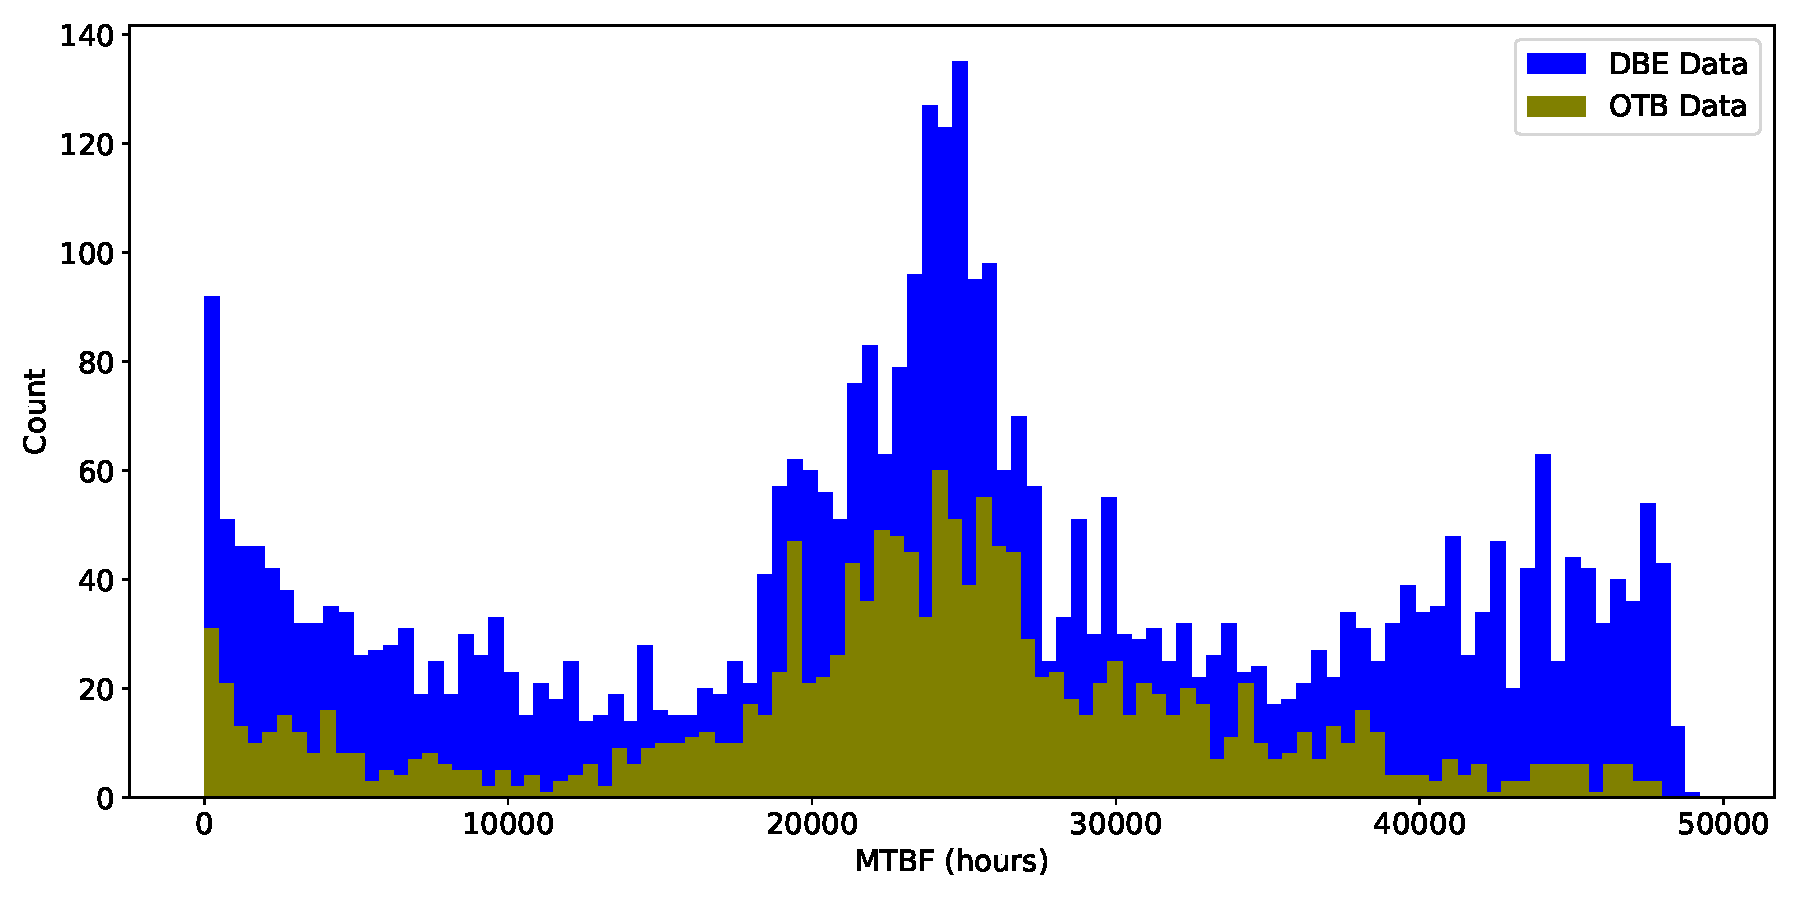
\includegraphics[width=\columnwidth]{figs/MTBF_GPUwise.pdf}
  \end{center}
  \caption{Distribution of device-level MTBFs due to DBE and OTB failures across all GPUs during the
entire lifetime of the machine. DBE and OTB events are separated for each GPU to distinguish between 
the failure pattern of each event type. Data includes both old and new batch of GPUs with the new ones 
mostly having MTBFs around or less than 3 years.}
  \label{fig:Device_MTBFs}
\end{figure}

Using the processed data, we analyze the inter-arrival times between the DBE and OTB events. 
This analysis is done at the device level and the system level. 
It provides important insights into the reliability of large-scale machines, where the 
failure rate of an individual device is significantly different from the overall reliability
of the machine.  

A histogram of MTBFs measured across GPUs which had at least one failure event is shown 
in Figure~\ref{fig:Device_MTBFs}. This is a practical assessment of device reliabilities 
as opposed to those provided in the device datasheet. The failures are tracked using the
SN of the GPUs even though a GPU might have been placed at different locations in the 
machine during its lifetime. The time to the first failure on a device is measured by taking
the insert time as the reference point, whereas, a simple difference is taken for subsequent
failures. It can be noticed that MTBFs due to DBE and OTB failures of most GPUs are clustered around 
25,000 hours or 2.8 years. This corresponds to the lifetime of most GPUs in the system after accounting 
for relocations and replacements done in the machine. The new batch of GPUs almost all of them lie below 
the average since most of them have a lifetime close to 3 years. It must be pointed out that the new batch did 
see a significantly less number of failures than the old batch as highlighted in the results presented later on.

Apart from the center cluster, a significant portion of GPUs have a very 
low MTBF (greater than zero and less than 1.5 hours) due to both DBE and OTB failures. 
This failure characteristic of the GPUs highlights a period when experiments 
were being done with putting the GPUs out of service on seeing a failure and moving them to new locations 
in the machine to possibly mitigate further failures. However, it turned out that the failures re-appeared 
even with putting the GPU in a new location. In some cases, the failures happened immediately after it is 
put into service at a different location. The use of insert time as a reference for first failure on a relocated
GPU to discount the out of service time and in some cases multiple back-to-back failures relatively immediately afterward,
cause a lot of GPUs to appear in the first bin of the histogram. These experiments continued until machine operators
figured out the root cause of the GPU failures as discussed earlier.  

On the other end of the spectrum, a noticeable portion of GPUs have very high
MTBFs due to DBE failures. This indicates the population of the GPUs that see a continuous operation in the machine 
despite its various episodes and see a single DBE event during their lifetime.
Apart from this behavior, the distribution of MTBF due to DBE events looks very similar to that due 
to OTB events. It can also be noted from Figure~\ref{fig:Device_MTBFs} that the number of recorded 
DBE events is significantly higher than the OTB events. This highlights the targeted replacement of GPUs 
with OTB events causing a substantial decrease in OTB events.  

%\begin{figure}[bt]
%  \begin{center}
%    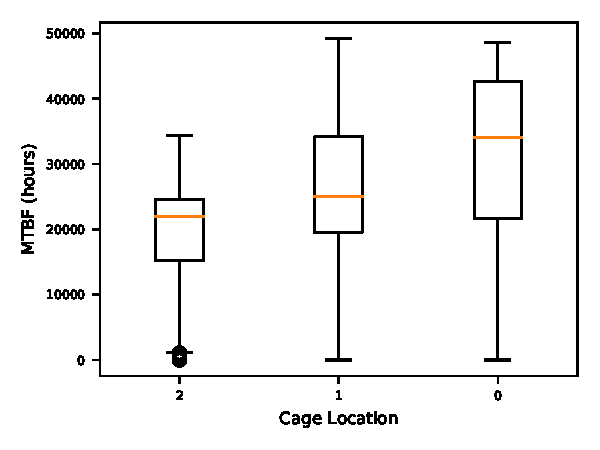
\includegraphics[width=\columnwidth]{figs/MTBF_CageWise.pdf}
%  \end{center}
%  \caption{MTBFs due to either DBEs or OTBs across the GPUs located in different cages.}
%  \label{fig:CageWise_MTBFs}
%\end{figure}

%\fix{Figure~\ref{fig:CageWise_MTBFs} shows temperature effect clearly. Should we move this 
%result to later in the paper?}

\begin{figure}[bt]
  \begin{center}
    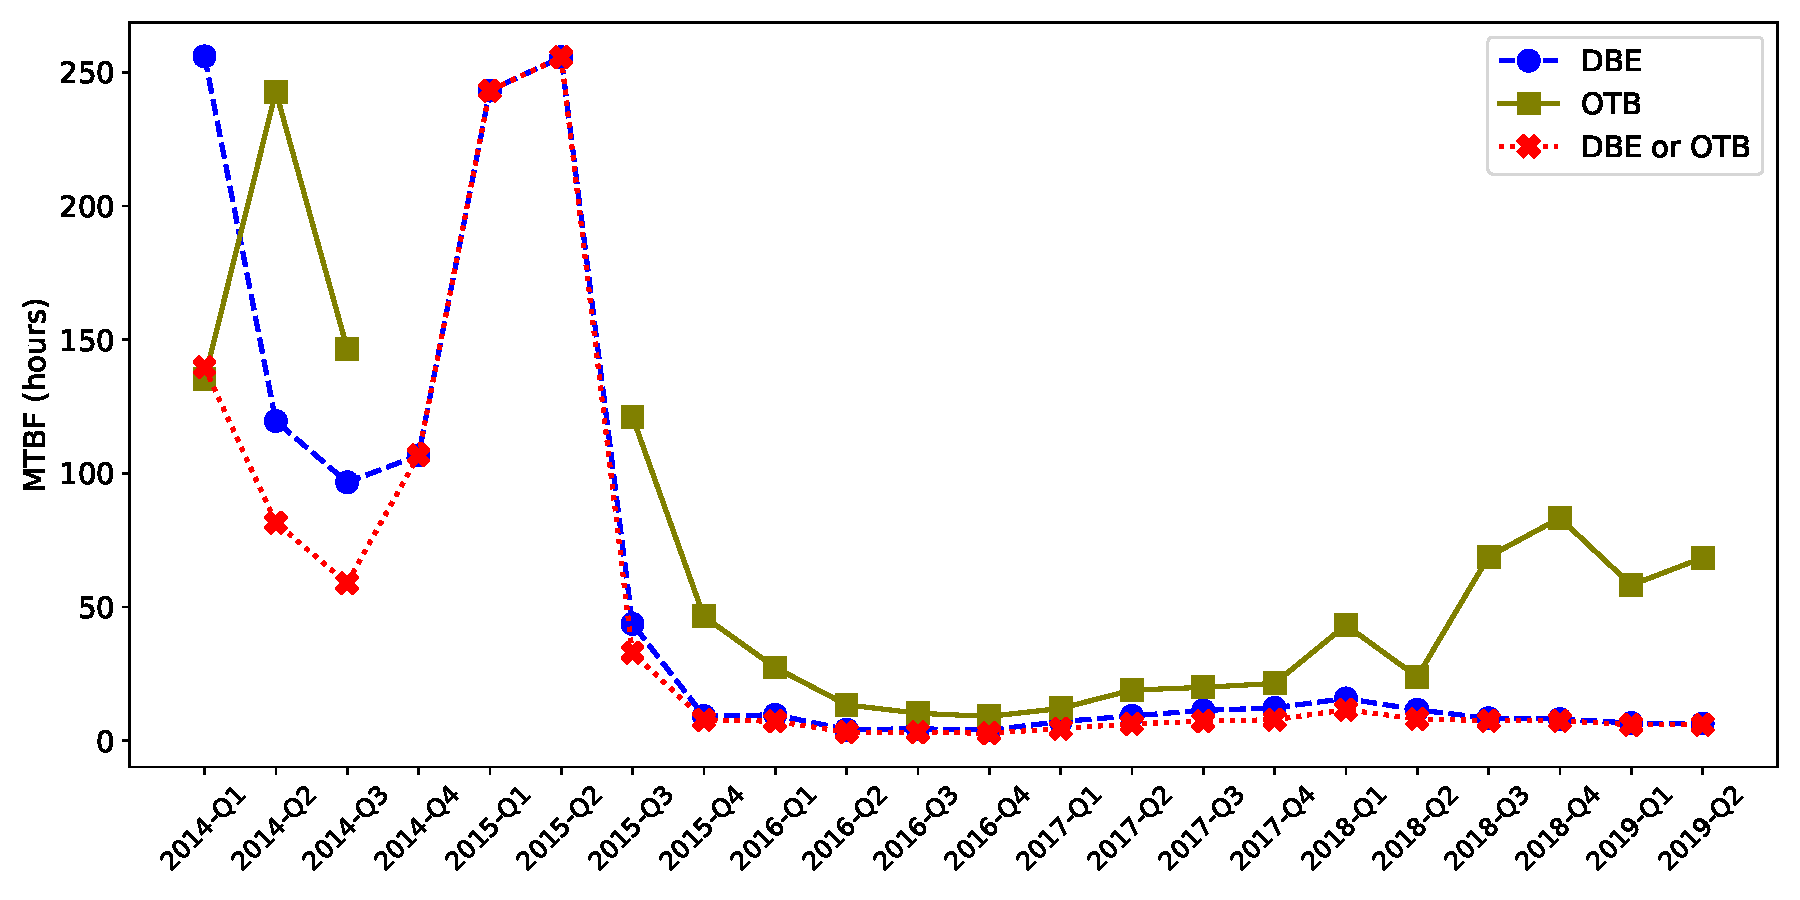
\includegraphics[width=\columnwidth]{figs/MTBF_quaterly_sys.pdf}
  \end{center}
  \caption{Variation of system-wide MTBF over the lifetime of the machine. System MTBF is calculated over 
three month periods to understand the various episodes of the machine. The three month periods are 
referred to as quarters, i.e., January through March is Q1, and so on. Most GPU replacements started taking 
place at the end of 2016-Q4 and were completed before 2018-Q1. DBE and OTB events are 
considered independently as well as together to represent failures occurring on the machine.}
  \label{fig:MTBF_sys}
\end{figure}

Although individual device MTBFs provide important insights into the varying failure rates
observed across the machine. It is worthwhile to perform a system-wide MTBF analysis since 
most high-performance computing applications use a significant number of GPUs in parallel. 
In the following analysis, failures occurring across all GPUs are consolidated and time between failures
is calculated. The old and new GPUs are all considered. At any given time, only a fixed number of GPUs
are in operation so any variation in time-between-failures is due to individual device reliabilities.

That said, a single MTBF number does not give an accurate picture of this machine.
With many GPU relocations and replacements across the machine over its lifetime, it is 
best to consider the variation of MTBF across fixed periods. Herein, we calculate 
the mean of time-between-failures across three months. Figure~\ref{fig:MTBF_sys}
clearly shows the considerable change in system-wide MTBF from one period to another. 
The observation of the MTBF trend shows the different phases which the machine went through. 
Relatively higher MTBFs are noted before 2015-Q4, with some quarters not having any OTB events 
and overall MTBF being determined solely by DBE events. During this phase, MTBF variation is seen
from quarter to quarter, but generally, system MTBF remains higher than a day (33 hours) and even reaches as high
as 10 days in one instance. An alarming drop in system MTBF to less than a day, i.e., 7.7 hours, is observed in 2015-Q4.
A consistent drop in system-wide MTBF is observed starting from 2015-Q2 until 2016-Q4. 
The corresponding increase in the number of failures during this phase can be seen in Figure~\ref{fig:NumFails_sys},
with the peak obtained in 2016-Q4. The usability of the machine comes into question with such low MTBFs, which triggered 
a phase of installing new GPUs in the machine.

When GPU replacements start to take place in late 
2016, it triggers a slight increase in MTBF. However, this change only lasts until 2018-Q1, when we see another 
downward trend of system MTBF. Incidentally, 2018-Q1 also marks the completion of all GPU replacements. 
So the upward trend noted in the period from 2016-Q4 to 2018-Q1 might be attributed to a portion of the machine 
being unavailable while the reworks were taking place. A single replacement cycle lasted multiple weeks. 
%\fix{need to verify how long the replacement took}
There is no definite way to incorporate this unavailability of the machine into MTBF analysis, so it has to
be said that overall there has been an increase in MTBF of the machine due to the replacements. 
For example, the lowest MTBF obtained in 2016-Q4 is 2.7 hours, with the subsequent periods having the 
lowest MTBF of 5.9 hours. With system MTBF less than a day, even slight variations in MTBF make it 
difficult to reliably run applications despite using failure recovery approaches such as checkpoint restart, 
as discussed later on in Section~\ref{section:discussion}. 

\begin{figure}[bt]
  \begin{center}
    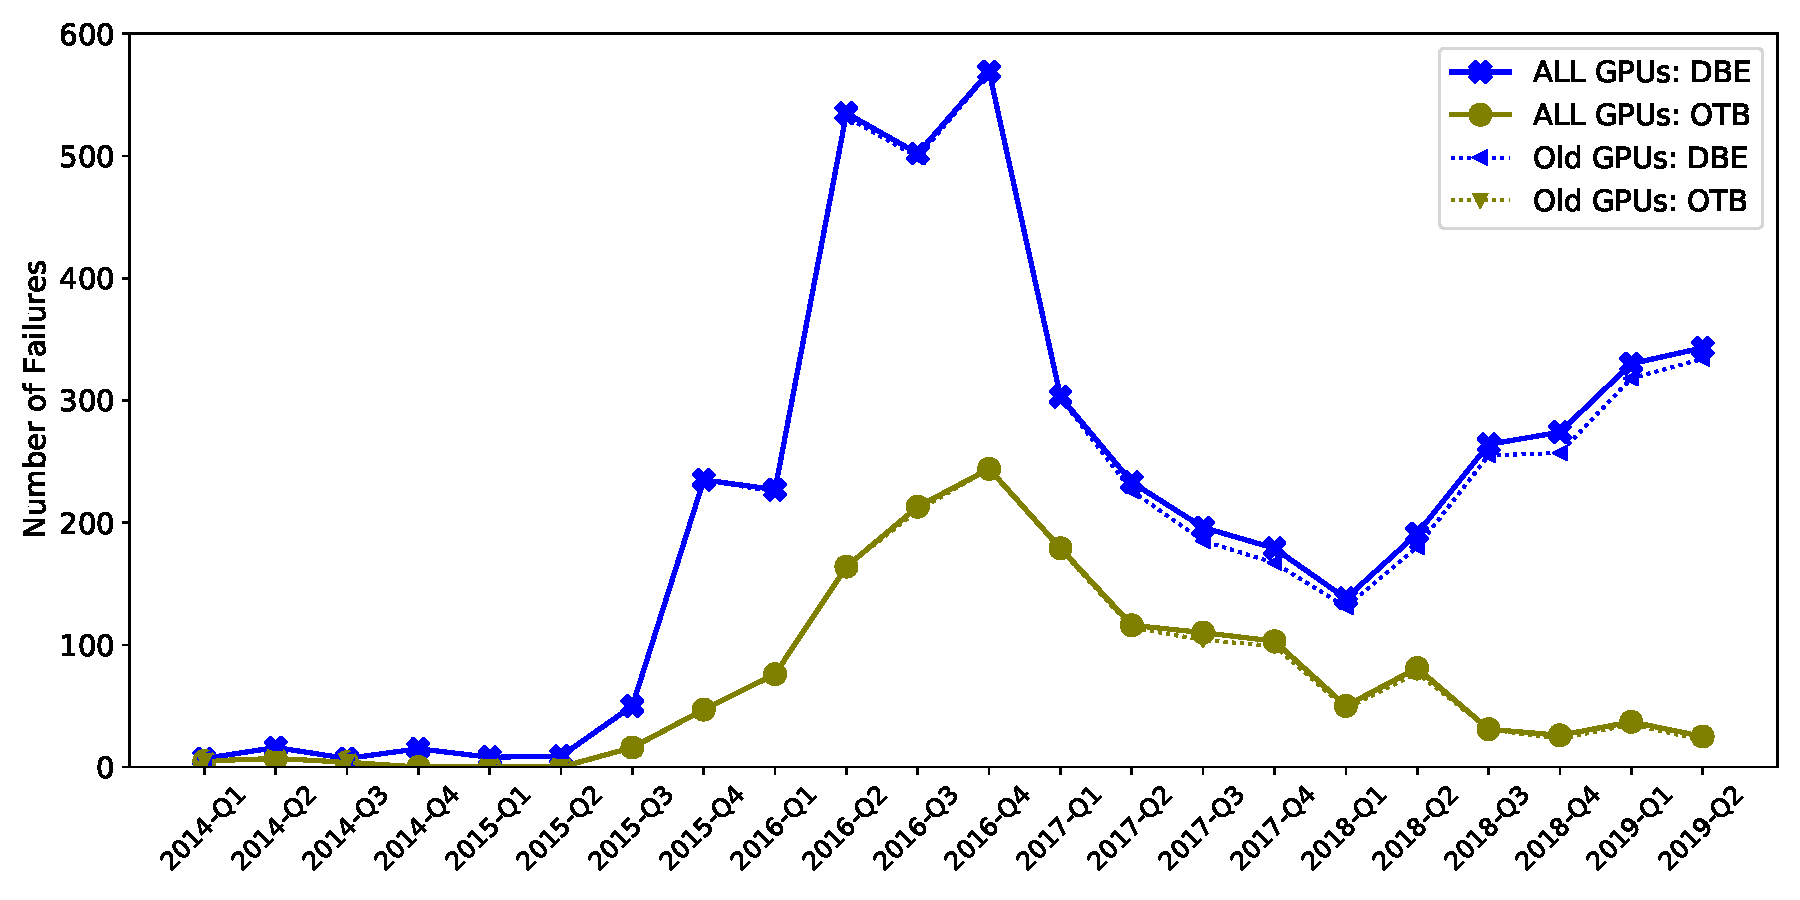
\includegraphics[width=\columnwidth]{figs/NumFailures_Quarterly_newOld.pdf}
  \end{center}
  \caption{The number of DBE and OTB failures observed over the lifetime of the machine.
A distinction is made for GPU failures happening across old GPUs to highlight the number
of failures across the newer GPUs. The peak failures are seen in 2016-Q4 (813 failures), 
which marked the commencement of major replacement of GPUs in the machine.}
  \label{fig:NumFails_sys}
\end{figure}

The mean-time-between DBE and OTB failures are also separately tracked in this analysis.
One observation is the drastic increase in mean-time-between OTB failures after the GPU replacements.
This is also evident from the reduction of the absolute number of OTB failures in Figure~\ref{fig:NumFails_sys}.
However, the system MTBF is determined by the weakest link and the occurrence of DBE events tends to dictate it.
Even though the replacements helped to increase the MTBF due to DBE events by a factor, the overall system 
reliability is dictated by the components with the most age in the system. There is a re-emergence of upward trend towards 
the end of life in the number of DBE failures in Figure~\ref{fig:NumFails_sys} which almost all of them are due to 
older GPUs in the system. 

\begin{figure}[bt]
  \begin{center}
    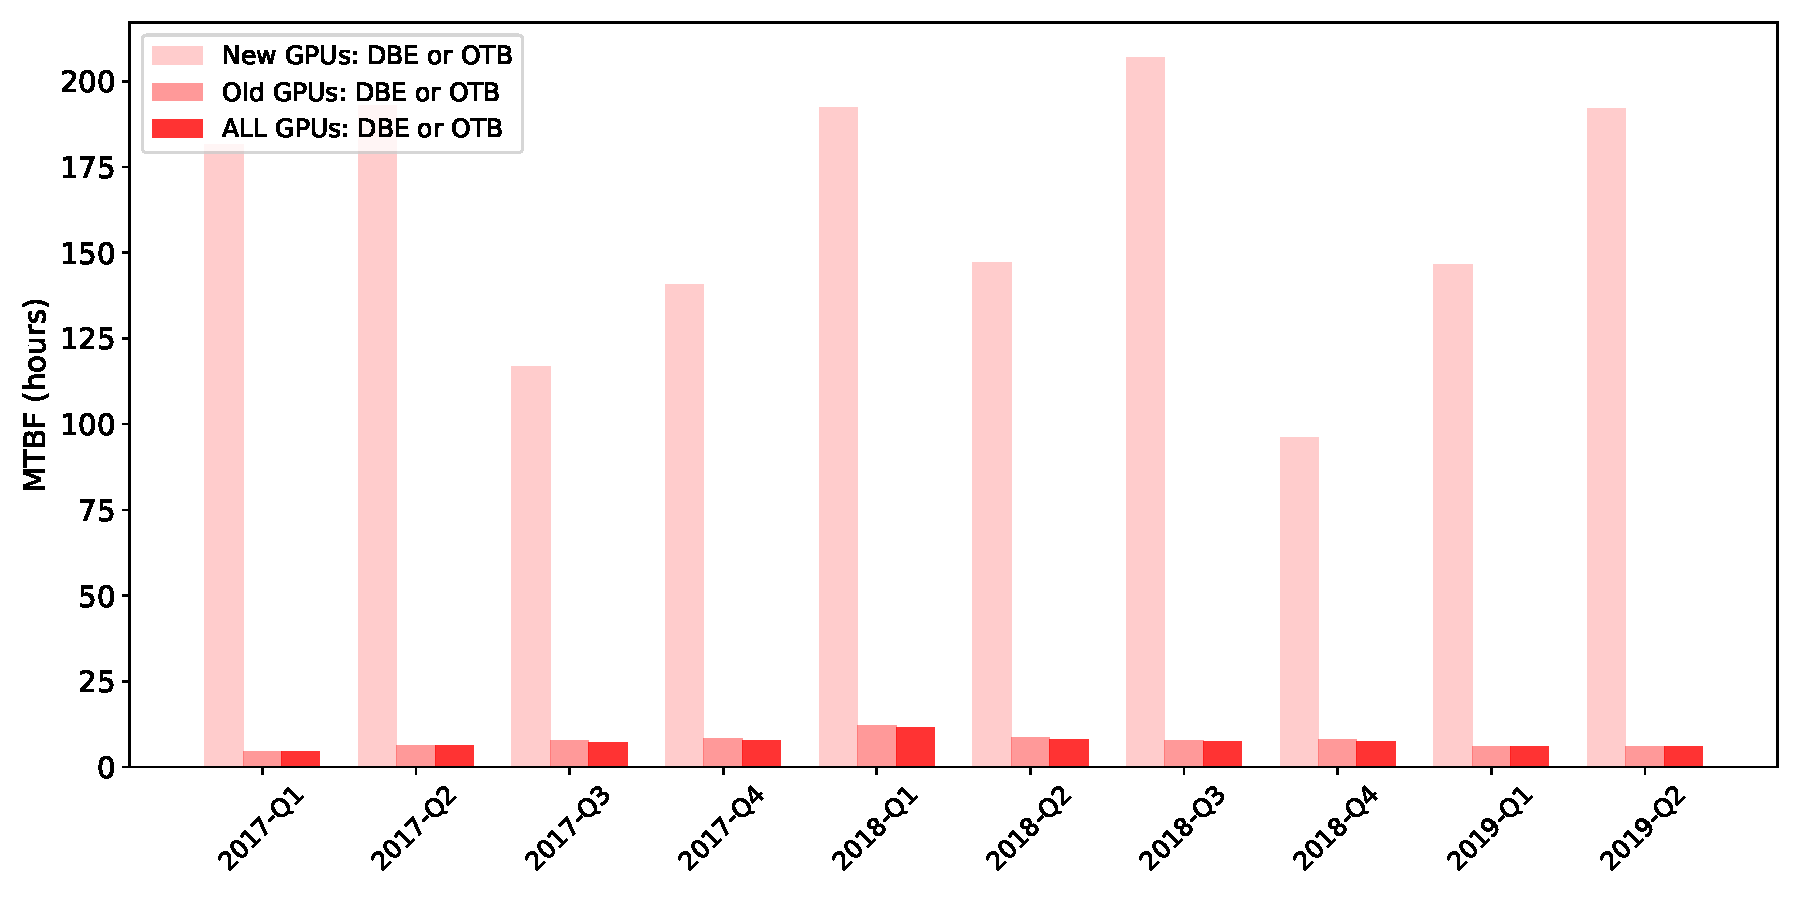
\includegraphics[width=\columnwidth]{figs/MTBF_quaterly_sys_NewOldALL.pdf}
  \end{center}
  \caption{Variation of system-wide MTBF across hypothetical new and old partitions of the machine over time.
Results are presented from 2017-Q1 which marked the beginning of when a substantial number of new GPUs are in service.
DBE and OTB events are both considered as a failure for calculating the MTBF.
Results highlight the difference in reliability observed by jobs using the new GPUs as compared to old GPUs,
as well as the minute difference in MTBF measured across the old partition and the whole machine.}
  \label{fig:MTBF_sys_NewOld}
\end{figure}

To better understand the difference in reliability of newer and old portions of the machine, 
Figure~\ref{fig:MTBF_sys_NewOld} shows the drastic difference in system MTBF measured in two hypothetical
partitions of the machine starting from the time when the majority of GPU replacements have been completed. 
The new partition of the machine has always 12X better MTBF than the older partition
of the machine. For example, in 2018-Q4, the MTBF recorded across old partition is about 7.9 hours, whereas it is about
96 hours (4 days) for the newer partition. The implications of such a huge disparity on applications running on the 
system are discussed in Section~\ref{section:discussion}. The insignificant difference in MTBF measured across all GPUs and
old partition of the machine can also be noted in Figure~\ref{fig:MTBF_sys_NewOld}.  
Therefore, the old GPUs that occupy a minority portion of the machine after GPU replacements, 
and have a disproportionately high number of failures and contribute towards a low system MTBF play a major role 
in determining the overall reliability of the machine.
The next section quantifies the survivability of this machine with its varied MTBF characteristics beyond its operational lifetime.
%\fix{George, can you please check the last sentence, where I make a connection with the next section.}

